\documentclass[paper=a4, english]{article}

\usepackage[T1]{fontenc}
\usepackage[utf8]{inputenc}
\usepackage{fourier}
\usepackage{geometry}
\geometry{verbose,tmargin=2.5cm,bmargin=2cm,lmargin=2.5cm,rmargin=2cm}
\usepackage{float}
\usepackage{textcomp}
\usepackage{amsmath}
\usepackage{stackrel}
\usepackage{graphicx}
\usepackage{esint}
\usepackage{tikz}
\usetikzlibrary{matrix,calc}

\makeatletter

\providecommand{\tabularnewline}{\\}

\usepackage{fancyhdr}
\usepackage{lscape}
\usepackage{amssymb}
\pagestyle{fancy}
\lhead{Electronica III - 22.13}
\chead{TPL1}
\rhead{ITBA}
\renewcommand{\headrulewidth}{1pt}
\renewcommand{\footrulewidth}{1pt}

\makeatother

\usepackage{babel}
\usepackage{listings}

\begin{document}

\section*{Task 1}

El progarma se invoca de la siguiente forma

\begin{lstlisting}
run a b c
\end{lstlisting}

Los parametros son:
\begin{itemize}
  \item $a$: Indica si el el sistema numerico será signado o no signado (0/1)
  \item $b$: Tamaño (en bits) de la parte entera del numero ($\geq0$)
  \item $c$: Tamaño (en bits) de la parte decimal del numero ($\geq0$)
\end{itemize}
Todos los inputs deben ser numeros. Además y c no puedn ser 0 a la vez
Todas estas restriciones son validadas

El problema usa formulas logicas simples para resolver el problema en los casos signados y no signados
La intuición detrás de las fórmulas se obtuvo observando la composición del número binario
\begin{figure}[H]
  \begin{centering}
  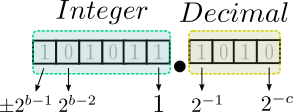
\includegraphics[scale=1]{bits.png}
  \par\end{centering}
  \caption{Visión del valor de cada bit}
\end{figure}
Como el bit menos significativo vale $2^{-c}$ luego la resolución es $2^{-c}$ y esto funciona tanto en el caso signado como en el no signado
\\
Sin embargo, para computar el rango debemos pensar en los dos casos por separado, mirando cuál es el más grande número (que llamaremos $r$) y el más chico número (que llamaremos $l$) que podemos formar en cada caso
En el caso no signado el número más chico es 0, y el más grande será
$$r=\underbrace{2^{-c}+2^{-c+1}+...+2^{-1}}_{1-2^{-c}}+\underbrace{1+2^{1}+...+2^{b-1}}_{2^{b}-1}=2^{b}-2^{-c}$$
Por lo tanto la resolución será $r-l=2^{b}-2^{-c}$
\\
Para el caso signado notamos que el numero más chico es cuando solo el bit más significativo es 1
$$l=-2^{b-1} $$
Y el más grande es cuando todos los bits son 1 excepto el más significativo
$$r=2^{-c}+2^{-c+1}+...+2^{1}+1+2^{1}+...+2^{b-2}=2^{b-1}-2^{-c}$$
Por lo tanto la resolución es $r-l=2^{b-1}-2^{-c}+2^{b-1}=2^{b}-2^{-c}$
Que es la misma, lo cual es razonable ya que podemos expresar la misma cantidad de numeros con la misma catndidad de bits y esto no depende si el sistema es o no signado
\end{document}
